% ------------------------------------------------------------------------
% ------------------------------------------------------------------------
% Modelo de relatório de estágio DAS - UFSC.
% Esse modelo usa abnTeX2 (https://www.abntex.net.br/)
% ------------------------------------------------------------------------
% ------------------------------------------------------------------------

\documentclass[
	% -- opções da classe memoir --
	12pt,				% tamanho da fonte
	openright,			% capítulos começam em pág ímpar (insere página vazia caso preciso)
	oneside,			% Para impressão simples. Para impressão frente e verso, use twoside
	a4paper,			% tamanho do papel. 
	% -- opções do pacote babel --
	english,			% idioma adicional para hifenização
	brazil				% o último idioma é o principal do documento
	]{abntex2}

% ---
% Pacotes básicos 
% ---
\usepackage{lmodern}			% Usa a fonte Latin Modern			
\usepackage[T1]{fontenc}		% Selecao de codigos de fonte.
\usepackage[utf8]{inputenc}		% Codificacao do documento (conversão automática dos acentos)
\usepackage{lastpage}			% Usado pela Ficha catalográfica
\usepackage{indentfirst}		% Indenta o primeiro parágrafo de cada seção.
\usepackage{color}				% Controle das cores
\usepackage{graphicx}			% Inclusão de gráficos
\usepackage{microtype} 			% para melhorias de justificação
% ---
		
% ---
% Pacotes de citações
% ---
\usepackage[brazilian,hyperpageref]{backref}	 % Paginas com as citações na bibl
\usepackage[alf]{abntex2cite}	% Citações padrão ABNT

% --- 
% CONFIGURAÇÕES DE PACOTES
% --- 

% ---
% Configurações do pacote backref
% Usado sem a opção hyperpageref de backref
\renewcommand{\backrefpagesname}{Citado na(s) página(s):~}
% Texto padrão antes do número das páginas
\renewcommand{\backref}{}
% Define os textos da citação
\renewcommand*{\backrefalt}[4]{
	\ifcase #1 %
		Nenhuma citação no texto.%
	\or
		Citado na página #2.%
	\else
		Citado #1 vezes nas páginas #2.%
	\fi}%
% ---

% ---
% Informações de dados para CAPA e FOLHA DE ROSTO
% ---
\titulo{Extração Transformação e Carregamento de dados: extração via coordenadas de arquivos}
\autor{Daniel Floriani da Silva}
\local{Florianópolis}
\data{2026}
\orientador{Leandro Buss Becker}
\coorientador{} % Deixar vazio caso não haja
\instituicao{%
  UNIVERSIDADE FEDERAL DE SANTA CATARINA
  \par
  CENTRO TECNOLÓGICO
  \par
  DEPARTAMENTO DE AUTOMAÇÃO E SISTEMAS}
\tipotrabalho{Relatório de Estágio}

\preambulo{Relatório submetido à Universidade Federal de Santa Catarina como requisito para a aprovação na disciplina \textbf{DAS 5501 - Estágio em Controle e Automação Industrial} do curso de Graduação em Engenharia de Controle e Automação.}
% ---

% ---
% Configurações de aparência do PDF final

% alterando o aspecto da cor azul
\definecolor{blue}{RGB}{41,5,195}

% informações do PDF
\makeatletter
\hypersetup{
     	%pagebackref=true,
		pdftitle={\@title}, 
		pdfauthor={\@author},
    	pdfsubject={\imprimirpreambulo},
	    pdfcreator={LaTeX with abnTeX2},
		pdfkeywords={abnt}{latex}{abntex}{abntex2}{trabalho acadêmico}, 
		colorlinks=true,       		% false: boxed links; true: colored links
    	linkcolor=black,          	% color of internal links
    	citecolor=blue,        		% color of links to bibliography
    	filecolor=magenta,      		% color of file links
		urlcolor=blue,
		bookmarksdepth=4
}
\makeatother
% --- 

% --- 
% Espaçamentos entre linhas e parágrafos 
% --- 

% O tamanho do parágrafo é dado por:
\setlength{\parindent}{1.3cm}

% Controle do espaçamento entre um parágrafo e outro:
\setlength{\parskip}{0.2cm}  % tente também \onelineskip

% ---
% compila o indice
% ---
\makeindex
% ---

% ----
% Início do documento
% ----
\begin{document}

% Retira espaço extra obsoleto entre as frases.
\frenchspacing 

% ----------------------------------------------------------
% ELEMENTOS PRÉ-TEXTUAIS
% ----------------------------------------------------------
% \pretextual

% ---
% Capa
% ---

\renewcommand{\imprimircapa}{%
  \begin{capa}%
    \center
    \ABNTEXchapterfont\Large\textbf\imprimirinstituicao
    
    \vspace*{1cm}
    
    {\ABNTEXchapterfont\large\textbf\imprimirautor}
    
    \vfill
    \begin{center}
    \ABNTEXchapterfont\bfseries\ Relatório de Estágio \\
    \ABNTEXchapterfont\bfseries\LARGE\imprimirtitulo
    \end{center}
    \vfill
    
    \large\imprimirlocal
    
    \large\imprimirdata
    
    \vspace*{1cm}
  \end{capa}
}

\imprimircapa
% ---

% ---
% Folha de rosto
% (o * indica que haverá a ficha bibliográfica)
% ---
\makeatletter
\renewcommand{\folhaderostocontent}{
  \begin{center}
  
    {\ABNTEXchapterfont\large\textbf\imprimirautor}
    
    \vspace*{\fill}\vspace*{\fill}
    
    \begin{center}
    	\ABNTEXchapterfont\bfseries\Large\imprimirtitulo
    \end{center}
    
    \vspace*{\fill}
    
    \abntex@ifnotempty{\imprimirpreambulo}{%
      \hspace{.45\textwidth}
      \begin{minipage}{.5\textwidth}
      \SingleSpacing
      \imprimirpreambulo
      \par
      {\imprimirorientadorRotulo~\imprimirorientador\par}
      \abntex@ifnotempty{\imprimircoorientador}{%
    	{\imprimircoorientadorRotulo~\imprimircoorientador}%
      }%
      \end{minipage}%
      \vspace*{\fill}
    }%
    
    \vspace*{\fill}
    
    {\large\imprimirlocal}
    
    \par
    
    {\large\imprimirdata}
    
    \vspace*{1cm}
  \end{center}
}
\makeatother

\imprimirfolhaderosto
% ---

% ---
% Inserir folha de aprovação
% ---

% Isto é um exemplo de Folha de aprovação, elemento obrigatório da NBR
% 14724/2011 (seção 4.2.1.3). Você pode utilizar este modelo até a aprovação
% do trabalho. Após isso, substitua todo o conteúdo deste arquivo por uma
% imagem da página assinada pela banca com o comando abaixo:
%
% \includepdf{folhadeaprovacao_final.pdf}
%
\makeatletter
\begin{folhadeaprovacao}

  \begin{center}
    {\ABNTEXchapterfont\large\imprimirautor}

    \vspace*{\fill}\vspace*{\fill}
    \begin{center}
      \ABNTEXchapterfont\bfseries\Large\imprimirtitulo
    \end{center}
    \vspace*{\fill}
    
    Este relatório de estágio foi julgado no contexto da disciplina DAS5501: Estágio em Controle e Automação Industrial e \textbf{APROVADO} na sua forma final pelo Curso de Engenharia de Controle e Automação.
    
    \vspace*{\fill}
    
    Florianópolis, 15 de abril de 2026
  \end{center}
  
   \assinatura{\textbf{\imprimirorientador} \\ Orientador \\ Universidade Federal de Santa Catarina}
   
   \assinatura{\textbf{Vinicius Rios Fuck} \\ Supervisor na Empresa \\ EMPRESA}
      
   \abntex@ifnotempty{\imprimircoorientador}{%
     \assinatura{\textbf{\imprimircoorientador} \\ Co-orientador \\ Universidade Federal de Santa Catarina}
   }%
\makeatother
   
        
\end{folhadeaprovacao}

% ---

% ---
% RESUMOS
% ---

% resumo em português
\setlength{\absparsep}{18pt} % ajusta o espaçamento dos parágrafos do resumo
\begin{resumo}
	O presente relatório de estágio descreve o desenvolvimento de uma solução automatizada para a empresa Veeries, organização que atua no setor do agronegócio oferecendo produtos de análise de mercado e fluxo de \textit{commodities}. O problema central abordado foi o severo gargalo operacional na ingestão de dados oriundos de relatórios em formato PDF de duas fontes externas confidenciais. Tal extração era executada de forma estritamente manual pela equipe de analistas, consumindo cerca de três horas por lote e apresentando alta suscetibilidade a falhas humanas e estruturais. Para solucionar este desafio tecnológico e de negócio, foi projetado e implementado um \textit{pipeline} de dados orientado a eventos, fundamentado na Arquitetura \textit{Medallion} (composto pelas camadas progressivas \textit{Bronze, Silver} e \textit{Gold}) e construído na linguagem Python, com suporte das bibliotecas Pandas e Pandera. O fluxo automatizou a extração bruta do formato não estruturado e implementou rigorosos Contratos de Dados (\textit{schemas}) para validações matemáticas e semânticas, além de adotar uma estratégia arquitetural de interrupção imediata em caso de anomalias estruturais (\textit{fail-fast}). Como resultado direto da implantação, o tempo de processamento de um lote de relatórios foi reduzido de horas para um intervalo de 2 a 5 segundos. A esteira automatizada transferiu a responsabilidade técnica integralmente para a equipe de desenvolvedores, livrou os analistas de mercado de tarefas braçais de transcrição e conferiu alta governança, rastreabilidade e resiliência ao banco de dados da organização. O sistema provou-se capaz de interceptar e bloquear erros de publicação oriundos das próprias fontes emissoras antes que alcançassem as ferramentas analíticas e de tomada de decisão da diretoria.

\vspace{\onelineskip}
\noindent
\textbf{Palavras-chave:} Engenharia de Dados. Arquitetura \textit{Medallion}. \textit{Pipeline} de Dados. Qualidade de Dados. Automação.
\end{resumo}

% resumo em inglês
\begin{resumo}[Abstract]
 \begin{otherlanguage*}{english}
	This internship report describes the development of an automated solution for Veeries, an organization operating in the agribusiness sector that offers market analysis and commodity flow products. The core problem addressed was the severe operational bottleneck in the data ingestion of PDF reports from two confidential external sources. This extraction was performed strictly manually by the analyst team, consuming about three hours per batch and presenting a high susceptibility to human and structural failures. To solve this technological and business challenge, an event-driven data pipeline was designed and implemented based on the Medallion Architecture (composed of progressive Bronze, Silver, and Gold layers) and built in Python, supported by Pandas and Pandera libraries. The workflow automated the raw extraction from the unstructured format and implemented strict Data Contracts (schemas) for mathematical and semantic validations, in addition to adopting an architectural strategy of immediate interruption in case of structural anomalies (fail-fast). As a direct result of the deployment, the processing time of a report batch was reduced from hours to an interval of 2 to 5 seconds. The automated pipeline transferred the technical responsibility entirely to the developers' team, freed market analysts from manual transcription tasks, and provided high governance, traceability, and resilience to the organization's database. The system proved capable of intercepting and blocking publication errors from the issuing sources themselves before they reached the analytical and decision-making tools of the board.

\vspace{\onelineskip}
\noindent
\textbf{Key-words:} Data Engineering. Medallion Architecture. Data Pipeline. Data Quality. Automation.
 \end{otherlanguage*}
\end{resumo}

% Inserir listas. Todas essas listas são opcionais.
\input{listas.tex}

% ---
% inserir o sumario
% ---
\pdfbookmark[0]{\contentsname}{toc}
\tableofcontents*
\cleardoublepage
% ---



% ----------------------------------------------------------
% ELEMENTOS TEXTUAIS
% ----------------------------------------------------------
\textual

% ----------------------------------------------------------
% Introdução (exemplo de capítulo sem numeração, mas presente no Sumário)
% ----------------------------------------------------------
\chapter*[Introdução]{Introdução}
\addcontentsline{toc}{chapter}{Introdução}
% ----------------------------------------------------------

Durante o estágio realizado na Veeries, entre outubro de 2025 e abril de 2026, identificou-se a necessidade de reestruturar a ingestão de dados de fontes externas críticas para o negócio (confidencial). 
O problema central era a ausência de um fluxo de dados padronizado, o que comprometia a rastreabilidade e a confiabilidade das informações consumidas pelas áreas de análise.
Para solucionar essa questão, atuei diretamente no desenvolvimento de um pipeline de dados automatizado, aplicando fundamentos de automação de processos do curso de Engenharia de Controle e Automação.

\section*{Objetivos e Metodologia}

O objetivo geral do projeto foi desenvolver um fluxo robusto de extração, processamento e disponibilização de dados.
Como objetivos específicos, destaco a construção do fluxo baseada na Arquitetura Medallion (camadas Bronze, Silver e Gold) e a implementação de rigorosas validações de qualidade estrutural.
\section*{Estrutura do Relatório}
Para relatar o desenvolvimento e os resultados alcançados, este documento está organizado da seguinte forma:
\begin{itemize}
    \item Capítulo 2: Descreve o contexto da empresa e detalha o problema enfrentado com os dados.
    \item Capítulo 3: Apresenta brevemente os conceitos da Arquitetura Medallion e as técnicas de validação utilizadas.
    \item Capítulo 4: Expõe a implementação técnica da solução, detalhando a codificação do pipeline (L0 a L2).
    \item Capítulo 5 e 6: Apresentam os resultados obtidos, a análise crítica dos impactos gerados e as considerações finais.
\end{itemize}


\begin{itemize}
\item 	definição do assunto, o problema a ser abordado no trabalho;
\item 	localização do assunto no espaço, no tempo e no contexto do Curso;
\item 	importância do assunto e justificativa da escolha;
\item 	objeto geral e objetivos específicos;
\item 	hipóteses levantadas ou argumentação principal;
\item 	descrição da metodologia empregada no trabalho (bibliografia e/ou estudo de campo e/ou de laboratório);
\item 	as alternativas de solução do Problema, decorrentes de estudo bibliográfico que deverá ficar evidenciado mediante referências;
\item 	apresentação do plano adotado para o desenvolvimento do assunto, isto é, a descrição do que será tratado em cada um dos capítulos subsequentes.
\end{itemize}




% Desenvolvimento
\input{desenvolvimento/capitulo1.tex}
\chapter{Capítulo 2}

A Veeries é uma empresa inserida no agronegócio. 
Oferece produtos relacionados à análise da produção, fluxo e operações de commodities, bem como fluxo e operações dos suprimentos e infra-estrutura relacionados a este mercado. 

A empresa conta com cerca de 20 funcionários e pode ser subdividida em duas equipes: uma de Analistas de mercado e outra de desenvolvedores, como assim são chamados na organização. 
Próximo ao produto final, os analistas são responsáveis por analisar as informações coletadas, fazer projeções e montar relatórios. 
Estritamente ligados ao processamento da informação, o time de desenvolvedores é composto por engenheiros, cientistas da computação e estudantes de áreas correlatas. 
São responsáveis pela melhoria do processo, desde a obtenção dos dados até a apresentação ao cliente.

ETL, sigla para Extraction, Transform, Load (extração, transformação e carregamento) é o processo de integração de dados provindo de uma ou mais fontes de informação. 
Inclui processos de limpeza, organização, validação e carregamento em um repositório organizado e é util para consolidar e garantir dados brutos.

Os dados da fonte de informação, sobretudo o seu nível de organização, dita o quão complexo vai ser sua extração. 
O grau de dificuldade aumenta conforme diminui a clareza da estrutura da informação. 
Comumente é utilizada a classificação de dados estruturados, dados semi-estruturados e dados não estruturados. 
Dados estruturados (bancos de dados relacionais, planilhas excel por exemplo) costumam trazer pouco esforço de processamento por conter sua estrutura quase que pronta para consumo em ferramentas de análise.  
Dados semi-estruturados não se encaixam em tabelas mas possuem marcadores e metadados (tais como saída de leitura de sensores, JSON, XML, logs de sistemas, e-mails). 
Já os dados não estruturados não possuem formato definido (documentos de texto livre, PDFs, imagens, vídeos) e por isso exigem mais esforço no processamento.

Este projeto de ETL vai lidar com um tipo de dado que se classificaria entre dados não estruturados e semi-estruturados, pois a fonte de informação está disposta em tabelas documentadas em arquivos de texto PDF aonde é possível localizar a posição relativa dos elementos de texto  


Descrição da empresa, processos, layouts, problemas, indicadores existentes, etc.

No Capítulo 2, deve-se fazer uma descrição da empresa, processos, layouts, problemas, etc., ou seja, mais detalhadamente motivar e enquadrar o problema dentro do que proporão (a ser descrito no próximo capítulo).
\chapter{Aspectos Conceituais} 

Para solucionar o problema da extração manual e garantir a confiabilidade dos dados ingeridos pela Veeries, fez-se necessário o uso de padrões arquiteturais consolidados na área de engenharia de dados. Este capítulo apresenta, de forma prática, os conceitos de \textit{pipelines} de dados, a Arquitetura \textit{Medallion} e a utilização de \textit{schemas} como contratos de dados, fundamentando as escolhas técnicas implementadas na solução.

\section{Pipelines e Qualidade de Dados}

Um \textit{pipeline} de dados consiste em um conjunto automatizado de processos que realiza a extração, o processamento, a validação e o carregamento de informações de um sistema de origem para um ambiente de destino \cite{polisetty23}. Em oposição aos processos manuais e rudimentares, a adoção de fluxos automatizados garante a continuidade da informação e mitiga drasticamente a ocorrência de falhas humanas \cite{reis22}.

A qualidade dos dados (\textit{Data Quality}) é o objetivo central dessas rotinas estruturadas, sendo uma medida avaliada com base em fatores como precisão, completude, consistência e confiabilidade \cite{polisetty23}. No contexto do processamento de dados não estruturados e semi-estruturados — como a leitura e extração de tabelas em arquivos PDF —, a automação do fluxo é o primeiro passo obrigatório para estabelecer a confiabilidade do que será entregue à equipe de analistas.

\section{Arquitetura \textit{Medallion} e Fragmentação de Ingestão}

Para organizar o \textit{pipeline} de maneira escalável, de fácil manutenção e rastreável, optou-se pela utilização da Arquitetura \textit{Medallion}. Trata-se de um padrão de projeto de organização de dados que divide os arquivos e processamentos em camadas lógicas, com o objetivo de melhorar progressivamente a estrutura e a qualidade das informações a cada nova etapa \cite{databricks_medallion, gujjala_medallion}.

Nesta arquitetura, a transição e o refinamento dos dados ocorrem na seguinte divisão:

\begin{itemize}
    \item \textbf{Camada \textit{Bronze} (L0):} Consiste na camada inicial de armazenamento, atuando como o ambiente de ingestão bruta (\textit{raw data}). Para lidar com a complexidade da extração de dados não estruturados (como os arquivos PDF abordados neste projeto), esta camada foi arquiteturalmente fragmentada em duas subzonas: a \textbf{L0 Original} e a \textbf{L0 Revisada}. 
    
    A \textbf{L0 Original} opera como uma \textit{landing zone} (zona de pouso) estrita, onde os arquivos são mantidos em seu estado original e imutável, garantindo o registro histórico exato e a possibilidade de reprocessamento seguro em caso de falhas \cite{gorelik19}. Já a \textbf{L0 Revisada} recebe esses dados em uma etapa subsequente. A literatura técnica estabelece que a camada \textit{Bronze} pode comportar um algoritmo de \textit{parsing} mínimo focado estritamente em garantir a consistência do formato de armazenamento, sem a aplicação de regras de negócio \cite{gujjala_medallion}. Assim, a L0 Revisada converte os dados do PDF para um formato semi-estruturado bruto (como tabelas extraídas), facilitando a transição sem aplicar os filtros de limpeza estrutural que são exclusivos da próxima camada.
    
    \item \textbf{Camada \textit{Silver} (L1):} Trata-se da camada intermediária. Nela, os dados tabulares provenientes da L0 Revisada são submetidos a rigorosos processos de limpeza, padronização, deduplicação e, principalmente, validação contra contratos predefinidos. É o estágio onde a informação deixa de ser um dado bruto e passa a ser um dado confiável e estruturado \cite{gujjala_medallion}.
    
    \item \textbf{Camada \textit{Gold} (L2):} É a camada final de processamento do repositório. Os dados, já limpos e validados, são agregados e transformados conforme as regras abrangentes da organização, ficando otimizados e prontos para o consumo analítico \cite{databricks_medallion}.
\end{itemize}

\section{Camada de Apresentação (\textit{Views}) e Versatilidade}

Embora a camada \textit{Gold} finalize o tratamento da informação, a entrega direta de tabelas físicas aos usuários analistas pode gerar engessamento. Para solucionar isso, as modernas arquiteturas de engenharia de dados adotam uma Camada de Apresentação (frequentemente materializada através de \textit{Views} lógicas) operando sobre a camada \textit{Gold} \cite{reis22}. 

Uma diretriz de projeto fundamental adotada neste trabalho foi a de propagar o máximo de campos e informações viáveis extraídas da fonte primária até a camada anterior à apresentação (L2). A premissa central de preservar a abrangência e a granularidade atômica dos dados garante uma extrema versatilidade ao \textit{pipeline} \cite{kimball13}. 

Se o cliente final (analista de mercado) alterar seus requisitos de negócio e solicitar a visualização de uma coluna extraída do PDF que não havia sido prevista nos relatórios iniciais, essa arquitetura evita retrabalho. Como o dado já foi extraído da L0 Revisada, validado na L1 e preservado até a camada L2, não há necessidade de reconstruir os \textit{scripts} de ingestão: basta editar os limites da \textit{View} para passar a expor a nova métrica. Esse desacoplamento entre armazenamento estruturado e apresentação final eleva a resiliência operacional da solução.

\section{Contratos de Dados e \textit{Schemas}}

Um dos principais desafios na ingestão de arquivos externos é a mudança inesperada na estrutura original dos dados, como o reposicionamento de valores em um PDF. Para evitar que essas alterações corrompam silenciosamente os relatórios finais da empresa, utilizam-se os Contratos de Dados (\textit{Data Contracts}), que são acordos técnicos estritos definindo o formato, a estrutura e a tipagem esperada das informações na transição entre as camadas do \textit{pipeline} \cite{kleppmann17, armbrust20}.

A principal ferramenta lógica para impor o cumprimento desses contratos é o \textit{Schema} (Esquema). O \textit{schema} especifica claramente os nomes das colunas, os tipos de dados exigidos e as restrições de obrigatoriedade \cite{liao20}. 

Ao se aplicar a imposição de esquemas (\textit{schema enforcement}) na transição entre a L0 Revisada e a camada \textit{Silver}, o sistema atua como uma barreira de segurança: registros que não cumprem os requisitos estruturais preestabelecidos são bloqueados ou sinalizados para correção. Essa prática é essencial para lidar com a evolução estrutural dos dados, protegendo o sistema contra quebras e garantindo que apenas informações íntegras fluam para as \textit{Views} de apresentação \cite{armbrust20}.
\chapter{A Arquitetura da Solução} 

Para sanar o gargalo operacional imposto pela extração manual de dados não estruturados, foi concebida uma arquitetura baseada em eventos lógicos e armazenamento em nuvem. Este capítulo descreve conceitualmente o novo fluxo de informações da Veeries, detalhando o ambiente de execução, o ciclo de vida dos arquivos e a transição da granularidade dos dados através das camadas do \textit{pipeline}.

\section{Ambiente de Execução e Orquestração}

A infraestrutura de armazenamento do projeto foi estabelecida sobre o ecossistema de nuvem sincronizada da organização (utilizando as plataformas \textit{OneDrive/SharePoint}). Essa escolha garante alta disponibilidade e espelhamento nativo dos arquivos do \textit{pipeline} com as estações de trabalho da equipe.

Como as fontes externas não possuem uma data de publicação exata ou previsível para a emissão dos seus relatórios mensais em PDF, a adoção de um agendador de tarefas tradicional (baseado em tempo cronometrado) resultaria em execuções ociosas ou falhas por ausência de arquivos. Portanto, o acionamento do \textit{pipeline} baseia-se em uma arquitetura orientada a eventos, com orquestração sob demanda. 

O fluxo se inicia quando o analista responsável pelo monitoramento recebe o documento da fonte (via e-mail ou portais do mercado). O arquivo é então salvo de maneira padronizada no diretório de entrada inicial do \textit{pipeline} (denominado \texttt{01\_RAW}). Após o armazenamento, o usuário aciona a execução do processamento através de um \textit{bot} no aplicativo de mensagens \textit{Telegram}, o qual atua como o gatilho externo. Este \textit{bot} envia um comando (via \textit{webhook} ou requisição de API) que inicia a rotina de execução do repositório no \textit{GitHub}, transferindo o processamento pesado para o ambiente em nuvem da aplicação.

A \autoref{fig_arquitetura} ilustra o diagrama esquemático deste fluxo lógico, desde a captura dos dados crus até a sua disponibilização para os usuários analistas de mercado.

\begin{figure}[htb]
    \caption{\label{fig_arquitetura}Diagrama de Arquitetura do \textit{Pipeline Medallion}}
    \begin{center}
        % DICA: Substitua 'Example.png' pelo nome exato do seu arquivo de imagem na pasta 'imagens'
        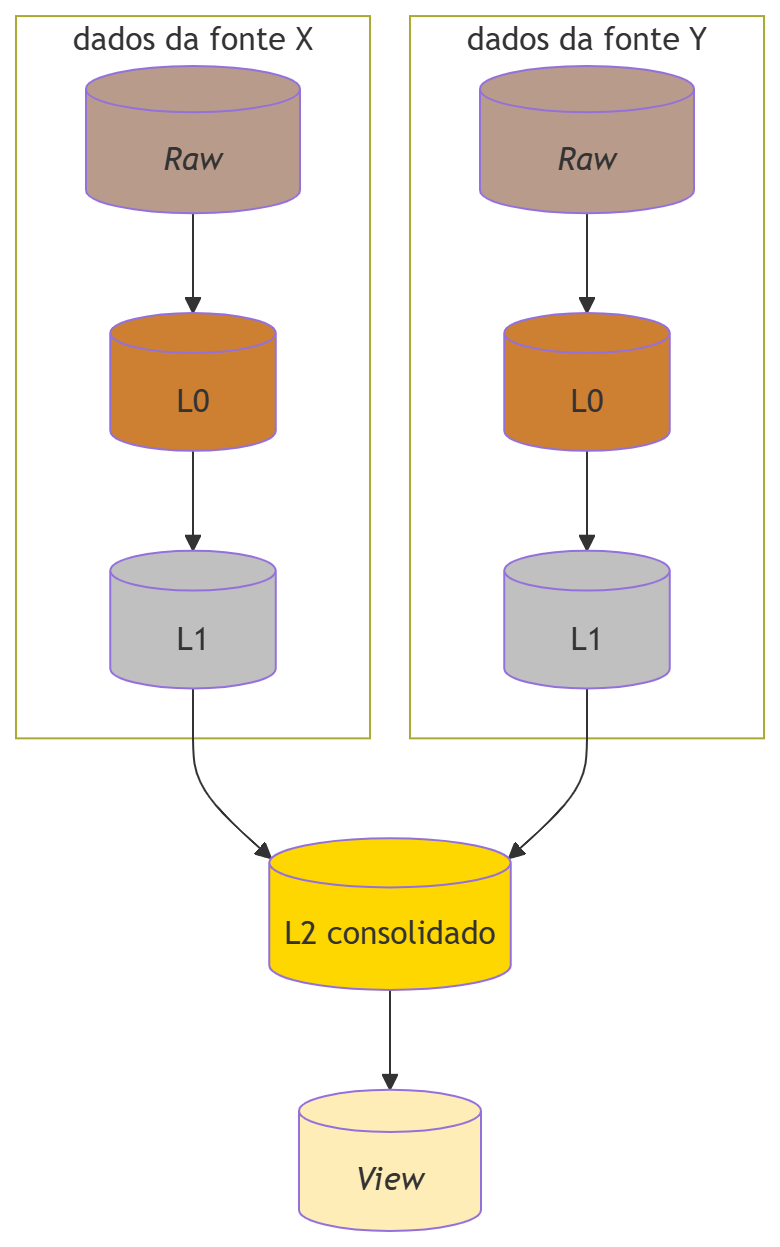
\includegraphics[scale=0.3]{imagens/arquitetura.png}
    \end{center}
    \legend{Fonte: Elaborado pelo autor.}
\end{figure}

\section{Fluxo e Evolução Estrutural dos Arquivos}

Uma diretriz central desta arquitetura foi o isolamento contínuo das fontes de dados durante as etapas de limpeza e validação, a fim de evitar que anomalias em um relatório comprometessem a ingestão do outro. A \autoref{fig_fluxo} detalha visualmente as etapas de processamento e a evolução estrutural dos arquivos dentro do \textit{pipeline}.

\begin{figure}[htb]
    \caption{\label{fig_fluxo}Fluxo de Processamento de Dados entre as Camadas}
    \begin{center}
        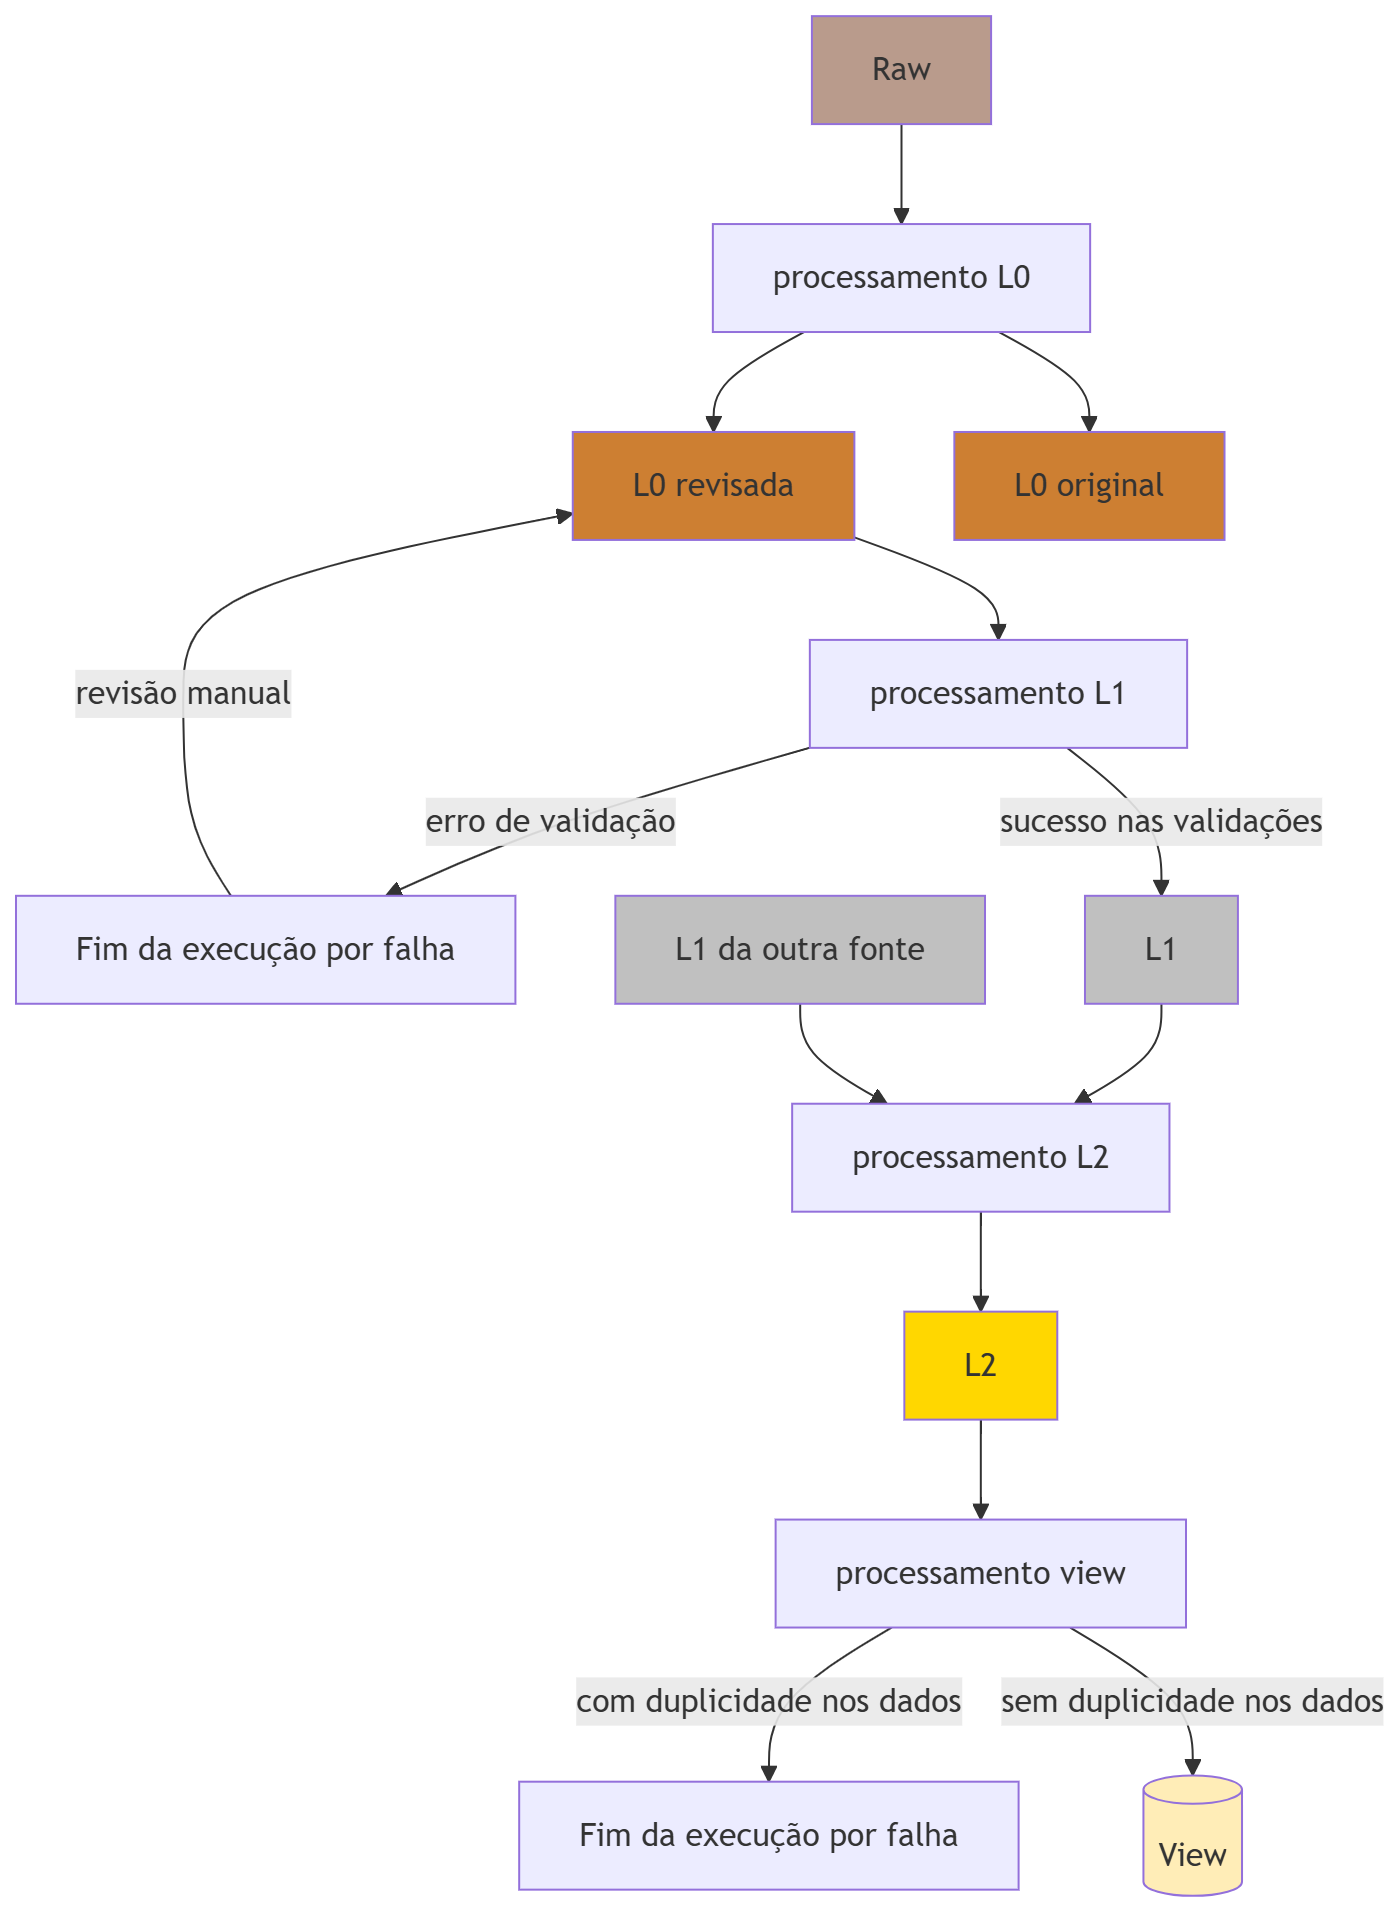
\includegraphics[scale=0.25]{imagens/fluxo_processamento.png}
    \end{center}
    \legend{Fonte: Elaborado pelo autor.}
\end{figure}

A transição e consolidação da informação ocorrem de maneira gradativa através das camadas:

\begin{itemize}
    \item \textbf{Camada \textit{Raw} (Crua):} Os arquivos que ingressam nesta camada preservam seu formato nativo (PDF). A granularidade é estritamente unitária: cada arquivo corresponde a um documento em PDF de uma única fonte de informação, retratando uma única data de emissão e um mês de referência específico. Os arquivos são mantidos em diretórios separados por fonte.
    
    \item \textbf{Camada \textit{Bronze} (L0 Original e Revisada):} Após o acionamento do \textit{parser}, o dado é convertido do formato PDF para arquivos tabulares (arquivos .CSV), preservando a granularidade original. Assim, na camada L0, cada CSV gerado continua representando os dados de uma única fonte para uma referência temporal específica. A fragmentação da L0 permite a tolerância a falhas na extração do texto antes de avançar para as validações estruturais.
    
    \item \textbf{Camada \textit{Silver} (L1):} A transição para a camada L1 engloba a imposição de esquemas e a validação matemática. A granularidade do arquivo sofre sua primeira alteração arquitetural: o arquivo gerado na camada L1 passa a representar a união consolidada de todos os arquivos históricos extraídos da L0 Revisada. Contudo, essa consolidação ainda ocorre de maneira particionada por fonte de informação. Isso garante que qualquer falha de validação ou processamento em uma das origens possa ser identificada e isolada sem interferir na disponibilidade dos dados da outra fonte.
    
    \item \textbf{Camada \textit{Gold} (L2):} É na penúltima camada de processamento que ocorre a consolidação global do \textit{pipeline}. Os dados validados das diferentes origens (Fonte X e Fonte Y) convergem para formar um único documento mestre de \textit{data warehouse}. A granularidade torna-se abrangente e multiorigem. 
\end{itemize}
\chapter{A Implementação do \textit{Pipeline}}

Este capítulo detalha a implementação técnica da solução arquitetada, traduzindo os conceitos lógicos e os fluxos de informação apresentados anteriormente em rotinas de código. O foco desta seção é expor o ambiente de desenvolvimento, a justificativa das tecnologias escolhidas e a estruturação algorítmica utilizada para transitar, validar e consolidar os dados através da Arquitetura \textit{Medallion}.

\section{Ambiente de Desenvolvimento e Tecnologias}

Todo o desenvolvimento do \textit{pipeline} foi realizado utilizando a linguagem de programação Python, escolhida por sua vasta adoção no ecossistema de dados, flexibilidade para lidar com arquivos não estruturados e robustez na manipulação tabular. 

Para estruturar as transformações, duas bibliotecas de código aberto foram fundamentais:
\begin{itemize}
    \item \textbf{Pandas:} Biblioteca primária de manipulação e análise de dados em Python. Foi utilizada em todas as camadas do projeto para operações de união, cálculos de subtotais e limpeza de \textit{strings}.
    \item \textbf{Pandera:} Biblioteca voltada especificamente para a validação estatística e estrutural de \textit{DataFrames} (estruturas tabulares de dados). O Pandera foi a tecnologia escolhida para materializar os "Contratos de Dados", garantindo a imposição de esquemas (\textit{schema enforcement}) durante a execução do código.
\end{itemize}

O código-fonte foi versionado utilizando a plataforma \textit{GitHub} e estruturado sob o paradigma de Programação Orientada a Objetos (POO), garantindo a modularidade e o reaproveitamento de rotinas entre diferentes fontes de dados.

\section{Orquestração e Ingestão (Camada \textit{Bronze})}

O fluxo de execução do projeto é coordenado por \textit{scripts} orquestradores (\texttt{main\_source.py}), responsáveis por acionar os módulos sequencialmente e interromper o processo imediatamente caso ocorra uma falha crítica em qualquer camada.

A primeira etapa do \textit{pipeline} é operada pelo módulo \texttt{l0\_process.py}. Este componente atua como o motor de ingestão da Camada \textit{Bronze} (L0). O seu papel principal é varrer os diretórios de entrada (\texttt{01\_RAW}), identificar novos relatórios em formato nativo (PDF ou planilhas despadronizadas) e acionar os algoritmos de extração de texto (\textit{parsers}). 

Optou-se por abstrair a complexidade visual dos relatórios nativos logo no momento da ingestão. O \textit{parser} localiza os dados tabulares e os metadados primários (como a data de referência do relatório) e o módulo L0 salva essas informações extraídas no formato CSV, mantendo a integridade exata do que foi lido (L0 Original). O armazenamento nesta camada utiliza um particionamento lógico em arquivos ZIP (compactados) organizados por ano e mês, otimizando o consumo de espaço em nuvem e facilitando a auditoria temporal.

\section{Validação e Padronização (Camada \textit{Silver})}

A transição para a Camada \textit{Silver} (L1) é o ponto crítico para a governança do \textit{pipeline}, sendo executada pelo módulo \texttt{l1\_process.py}. É nesta etapa que os dados brutos deixam de ser tratados apenas como "texto" e passam a ser validados como regras de negócio.

A implementação dessa validação baseia-se fortemente no arquivo \texttt{schemas.py}, onde classes de validação do \textit{Pandera} definem os contratos estruturais. Como exemplo, a classe \texttt{L1Schema} força que todas as instâncias possuam campos tipados corretamente (como datas de referência obrigatórias e colunas de identificação de origem). Caso a Fonte X altere a estrutura do seu relatório e o módulo de ingestão absorva colunas inesperadas, o processo de validação acusará uma violação de contrato e interromperá a execução, bloqueando a propagação do erro estrutural.

Além da tipagem, o módulo L1 realiza o mapeamento dos dados. Através da leitura de dicionários de conversão externos (arquivos do Excel gerenciados pela equipe de mercado), os nomes de produtos e variáveis que chegam despadronizados da fonte são normalizados para as nomenclaturas internas da Veeries, centralizando o controle semântico.

\section{Transformação Analítica e Apresentação (Camadas \textit{Gold} e \textit{View})}

O refino final dos dados é dividido entre os módulos \texttt{l2\_process.py} (Camada \textit{Gold}) e \texttt{view\_monthly\_process.py} (Camada de Apresentação).

Na camada L2, a rotina de código executa a principal alteração estrutural do dado: a operação de \textit{Melt} (despivoteamento). Essa técnica transforma colunas específicas (por exemplo, múltiplas colunas representando diferentes portos) em linhas, alterando a tabela para o formato longo (\textit{long format}). Esse formato é o padrão-ouro exigido por ferramentas modernas de visualização. É também nesta camada que são processadas as agregações lógicas (subtotais sintéticos de categorias de produtos) e aplicadas as validações estritas de unicidade (\textit{validate\_uniqueness}) para prevenir a multiplicação indevida de instâncias.

Por fim, o módulo \textit{View} abstrai toda a complexidade da engenharia para o usuário final. Ele atua removendo os metadados de auditoria e executa o filtro de versão cronológica (\textit{date versioning}). Caso as fontes emitam relatórios redundantes ou retificados no mesmo mês, o código utiliza a data de extração para deduplicar a base, garantindo que a versão entregue aos analistas reflita estritamente o cenário mais atual e fidedigno do mercado.
\chapter{Resultados e Discussões}

Este capítulo apresenta a análise crítica dos resultados obtidos com a implantação do \textit{pipeline} em ambiente de produção. O objetivo é avaliar a eficácia da solução proposta frente aos problemas de despadronização e morosidade detalhados no Capítulo 2, dimensionando os impactos quantitativos de desempenho e os ganhos qualitativos de governança de dados para a Veeries.

\section{Impacto Operacional e Dimensionamento do Processamento}

O benefício imediato e mais expressivo da automatização foi o ganho de eficiência temporal em escala. No paradigma anterior, a equipe dedicava cerca de 3 horas de trabalho humano aplicadas à leitura, transcrição e validação não estruturada em cada lote mensal de relatórios. Com a nova arquitetura, o tempo de extração, validação, cruzamento e consolidação dos dados despencou para um intervalo de execução entre 2 a 5 segundos.

Para dimensionar o impacto quantitativo da solução, a consolidação da base histórica processou de forma automatizada documentos abrangendo o período de janeiro de 2023 a fevereiro de 2026. Devido ao padrão de republicação retroativa da Fonte X, o \textit{pipeline} ingere um volume massivo de documentos: são 144 arquivos anuais apenas para esta origem (divididos entre publicações mensais e acumuladas), o que resulta em picos de até 23 relatórios processados simultaneamente em um único mês. A Fonte Y, de publicação linear, agregou 29 documentos históricos ao escopo.

Essa extração em larga escala gerou uma base rastreável de 24.588 registros consolidados na Camada \textit{Silver} (L1), sendo 23.270 provenientes da Fonte X e 1.318 da Fonte Y. Na Camada \textit{Gold} (L2), após a operação estrutural de despivoteamento (\textit{Melt}) das variáveis originais para 20 colunas de análise contínuas, o sistema computou um crescimento exponencial, validando 492.540 registros históricos no formato longo (sendo 238.260 registros mensais e 254.280 acumulados). 

Por fim, o filtro lógico de deduplicação da Camada \textit{View} cumpriu o seu papel de abstrair a redundância gerada pela sobreposição de relatórios da fonte, entregando 29.322 instâncias definitivas (28.584 da Fonte X e 738 da Fonte Y). O esforço da equipe, portanto, deixou de ser a transcrição braçal de arquivos e passou a ser o consumo imediato de uma base cronologicamente atualizada de quase 30 mil linhas fidedignas prontas para as ferramentas de \textit{Business Intelligence}.

\section{Governança, Resiliência e Tratamento de Exceções}

Sob a perspectiva qualitativa, a adoção da Arquitetura \textit{Medallion} e da estratégia \textit{fail-fast} (falhar rapidamente) provou-se altamente eficaz na proteção do ambiente analítico da empresa. Durante os ciclos de operação real, o sistema de monitoramento conseguiu identificar e barrar a propagação de anomalias que, no método manual, passariam despercebidas.

Com o novo fluxo, quando o \textit{pipeline} reporta uma interrupção de sucesso, o trabalho do desenvolvedor responsável restringe-se a investigar a causa apontada pelos \textit{logs} e atuar em três frentes principais de exceção:

\begin{itemize}
    \item \textbf{Produtos não mapeados:} Como os relatórios externos frequentemente introduzem categorias de produtos voláteis ou nomenclaturas inéditas, a validação de dicionário da camada \textit{Silver} (L1) barra o processamento instantaneamente. O desenvolvedor então apenas adiciona a nova instância ao dicionário central de mapeamento e reexecuta o código.
    \item \textbf{Inconsistências de estrutura nativa:} Quando a fonte altera ligeiramente a forma que publica os dados, o desenvolvedor realiza ajustes pontuais na camada L0 Revisada. Isso valida a premissa arquitetural discutida no Capítulo 3: é possível corrigir o formato de leitura sem perder a rastreabilidade original do documento preservado na L0 Original.
    \item \textbf{Auditoria de séries históricas e erros da fonte:} O impacto mais notável de qualidade de dados ocorreu durante a consolidação histórica das bases. As validações matemáticas identificaram o aparecimento de uma categoria de produto que não possuía sentido lógico na série temporal. A restrição estrutural revelou que a falha não era do algoritmo de extração, mas sim um erro de publicação da própria fonte externa emissora do relatório. 
\end{itemize}

O bloqueio automático desse erro de publicação externa comprova o sucesso primário deste projeto. A implementação não apenas resolveu o problema de lentidão, mas instituiu uma malha fina de confiabilidade sistêmica. A Veeries agora possui a garantia de que os relatórios que abastecem suas ferramentas de tomada de decisão (BI) são estritamente fidedignos e auditáveis, eliminando o risco do consumo de dados corrompidos.
\chapter{Considerações Finais e Perspectivas}

Este capítulo apresenta a síntese interpretada dos resultados alcançados ao longo do estágio, avaliando o cumprimento dos objetivos propostos. Discutem-se também as limitações inerentes à solução desenvolvida e são traçadas perspectivas para trabalhos futuros.

\section{Síntese e Avaliação dos Resultados}

O desenvolvimento deste \textit{pipeline} de extração e validação atingiu plenamente o objetivo de solucionar o gargalo operacional da Veeries. A substituição de um processo manual rudimentar, que consumia cerca de 3 horas de trabalho humano por lote de relatórios, por uma execução automatizada de até 5 segundos representa um ganho de eficiência evidente.

Do ponto de vista da governança, a adoção da Arquitetura \textit{Medallion} e a aplicação rigorosa de Contratos de Dados mostraram-se escolhas arquiteturais acertivas. O método implementado foi significativamente superior à abordagem anterior, não apenas pela velocidade de ingestão, mas pela capacidade de trazer robustez ao repositório de informações. O sistema transferiu a responsabilidade da equipe de uma atuação repetitiva e transcritora para um papel analítico e de curadoria de negócio. O bloqueio automático e bem-sucedido de anomalias e erros gerados pela própria fonte emissora atesta que o código desenvolvido entregou o nível máximo de confiabilidade exigido para a tomada de decisão da empresa.

\section{Limitações do Projeto}

Apesar do sucesso operacional, a solução atual opera sob alguns pressupostos lógicos e possui limitações que devem ser pontuadas:

\begin{itemize}
    \item \textbf{Dependência de Gatilho Humano:} Devido à imprevisibilidade na data e horário de publicação dos relatórios pelas fontes externas, o \textit{pipeline} ainda depende que o usuário (manutentor) identifique visualmente a disponibilidade do arquivo (via portal ou e-mail) e acione o processamento através do \textit{bot} no aplicativo \textit{Telegram}.
    \item \textbf{Suscetibilidade a Mudanças Estruturais Severas:} O algoritmo de extração de texto (\textit{parser}) foi desenhado para tolerar pequenas flutuações de margens e espaçamentos da fonte nativa. Contudo, se a entidade externa alterar drasticamente a disposição visual das tabelas no PDF, o sistema falhará intencionalmente (\textit{fail-fast}) para proteger a integridade dos dados, exigindo a intervenção nos métodos de captura dos dados nos arquivos brutos.
\end{itemize}

\section{Perspectivas e Trabalhos Futuros}

Uma vez que a estrutura algorítmica foi concebida sob o paradigma de Programação Orientada a Objetos e os módulos encontram-se rigorosamente desacoplados, a arquitetura oferece um vasto campo para evoluções. Como sugestões lógicas para a continuidade deste trabalho, destacam-se:

\begin{itemize}
    \item \textbf{Automação da Captura:} O desenvolvimento e integração de um módulo de RPA (\textit{Robotic Process Automation} - Automação Robótica de Processos) ou \textit{Web Scraping} (técnica de extração de dados da web) para monitorar continuamente as caixas de e-mail ou os portais das fontes. Essa evolução eliminaria o monitoramento humano, tornando todo o fluxo da informação 100\% autônomo.
    \item \textbf{Expansão Horizontal do Modelo:} Aproveitar as classes abstratas e as funções de padronização universal já codificadas (como as validações cruzadas e os \textit{schemas} de L1 e L2) para englobar dezenas de outras fontes nativas recebidas pela Veeries, padronizando progressivamente a ingestão de toda a organização sob o modelo \textit{Medallion}.
\end{itemize}


% ----------------------------------------------------------
% Finaliza a parte no bookmark do PDF
% para que se inicie o bookmark na raiz
% e adiciona espaço de parte no Sumário
% ----------------------------------------------------------
\phantompart

% ----------------------------------------------------------
% ELEMENTOS PÓS-TEXTUAIS
% ----------------------------------------------------------
\postextual
% ----------------------------------------------------------

% ----------------------------------------------------------
% Referências bibliográficas
% ----------------------------------------------------------
\bibliography{bibliografia}

% ----------------------------------------------------------
% Apêndices
% ----------------------------------------------------------

% ---
% Inicia os apêndices
% ---
\begin{apendicesenv}

\chapter{Glossário de termos técnicos}
\begin{itemize}
    \item \textbf{Arquitetura \textit{Medallion}:} Padrão de projeto de organização de dados que divide os arquivos em camadas lógicas (comumente chamadas de \textit{Bronze, Silver} e \textit{Gold}), com o objetivo de melhorar progressivamente a estrutura e a qualidade das informações a cada etapa do processamento.
    
    \item \textbf{Camada \textit{Bronze} (L0):} Camada inicial de armazenamento onde os dados brutos (\textit{raw data}) são mantidos em seu estado original, exatamente como foram extraídos das fontes, sem aplicação de filtros ou transformações estruturais.
    
    \item \textbf{Camada \textit{Silver} (L1):} Camada intermediária na qual os dados provenientes da camada \textit{Bronze} passam por processos de limpeza, padronização, deduplicação e validação de qualidade contra contratos predefinidos.
    
    \item \textbf{Camada \textit{Gold} (L2):} Camada final onde os dados, já limpos e validados, são agregados e transformados com base em regras de negócio específicas, ficando prontos e otimizados para o consumo analítico e a geração de relatórios.
    
    \item \textbf{Contrato de Dados (\textit{Data Contract}):} Acordo técnico e formal que define a estrutura, o formato, os padrões de qualidade e o comportamento esperado dos dados na transição entre sistemas ou camadas.
    
    \item \textbf{\textit{Parser}:} Algoritmo ou rotina desenvolvida para analisar uma estrutura de dados de entrada (como um arquivo de texto, CSV ou planilha) e extrair os parâmetros e informações relevantes de forma legível para o sistema.
    
    \item \textbf{\textit{Pipeline} de Dados:} Conjunto automatizado de processos e fluxos que realiza a extração, o processamento, a validação e o carregamento de dados de um sistema de origem para um ambiente de destino.
    
    \item \textbf{\textit{Schema} (Esquema):} Estrutura lógica que atua como a ferramenta de validação de um contrato de dados, especificando os nomes das colunas, os tipos de dados exigidos (como inteiro, texto ou data) e as restrições de obrigatoriedade.
\end{itemize}

\end{apendicesenv}
% ---


% ----------------------------------------------------------
% Anexos
% ----------------------------------------------------------

% ---
% Inicia os anexos
% ---
\begin{anexosenv}

% ---
\chapter{Título Opcional.}
% ---
Documentos não elaborados pelo autor, utilizados de fundamentação (mapas, leis, estatutos).

\end{anexosenv}

%---------------------------------------------------------------------
% INDICE REMISSIVO
%---------------------------------------------------------------------
\phantompart
\printindex
%---------------------------------------------------------------------

\end{document}
